%    JJJ    AA     CCCCCC KKK   K TTTTTT HH  HH EEEEEE BBBBBB UU  UU SSSSSS    CCCCCC OOOOOO MM  MM
%    JJJ   AAAA    CCCCCC KKK  K  TTTTTT HH  HH EEEEEE BB   B UU  UU SSS       CCCCCC OOOOOO MM  MM
%    JJJ  AA  AA   CC     KKK K     TT   HHHHHH EEE    BB   B UU  UU SSS       CC     OO  OO MMMMMM
%    JJJ AA    AA  CC     KKKK      TT   HHHHHH EEEEEE BBBBBB UU  UU  SSSSS    CC     OO  OO M MM M
%    JJJ AAAAAAAA  CC     KKK K     TT   HH  HH EEE    BB   B UU  UU    SSS    CC     OO  OO M MM M
% JJJJJJ AA    AA  CCCCCC KKK  K    TT   HH  HH EEEEEE BB   B UUUUUU    SSS .. CCCCCC OOOOOO M MM M
% JJJJJJ AA    AA  CCCCCC KKK   K   TT   HH  HH EEEEEE BBBBBB UUUUUU SSSSSS .. CCCCCC OOOOOO M MM M
% 
% Texte Geschrieben von Stefan Bopp und Chantal Frunz
% Mehr Informationen sind auf jackthebus.com zu finden


\section{Sinn und Zweck der Anleitung}
Die Anleitung soll eine Hilfe und Informationsquelle für alle darstellen. 
Die Systeme von Jack werden dank meiner Bastelleidenschaft nicht übersichtlicher.
Dies ist ein Versuch Ordnung zu schaffen und es anderen Personen ermöglichen den Bus auch zu betreiben.
Eine ausgedruckte Kopie dieses Dokuments befindet sich im Bus.
Die aktuelle Version ist hier zu finden:


\section{Elektrisches System}
\subsection{Schema}

\begin{figure}[H]
    \centering
    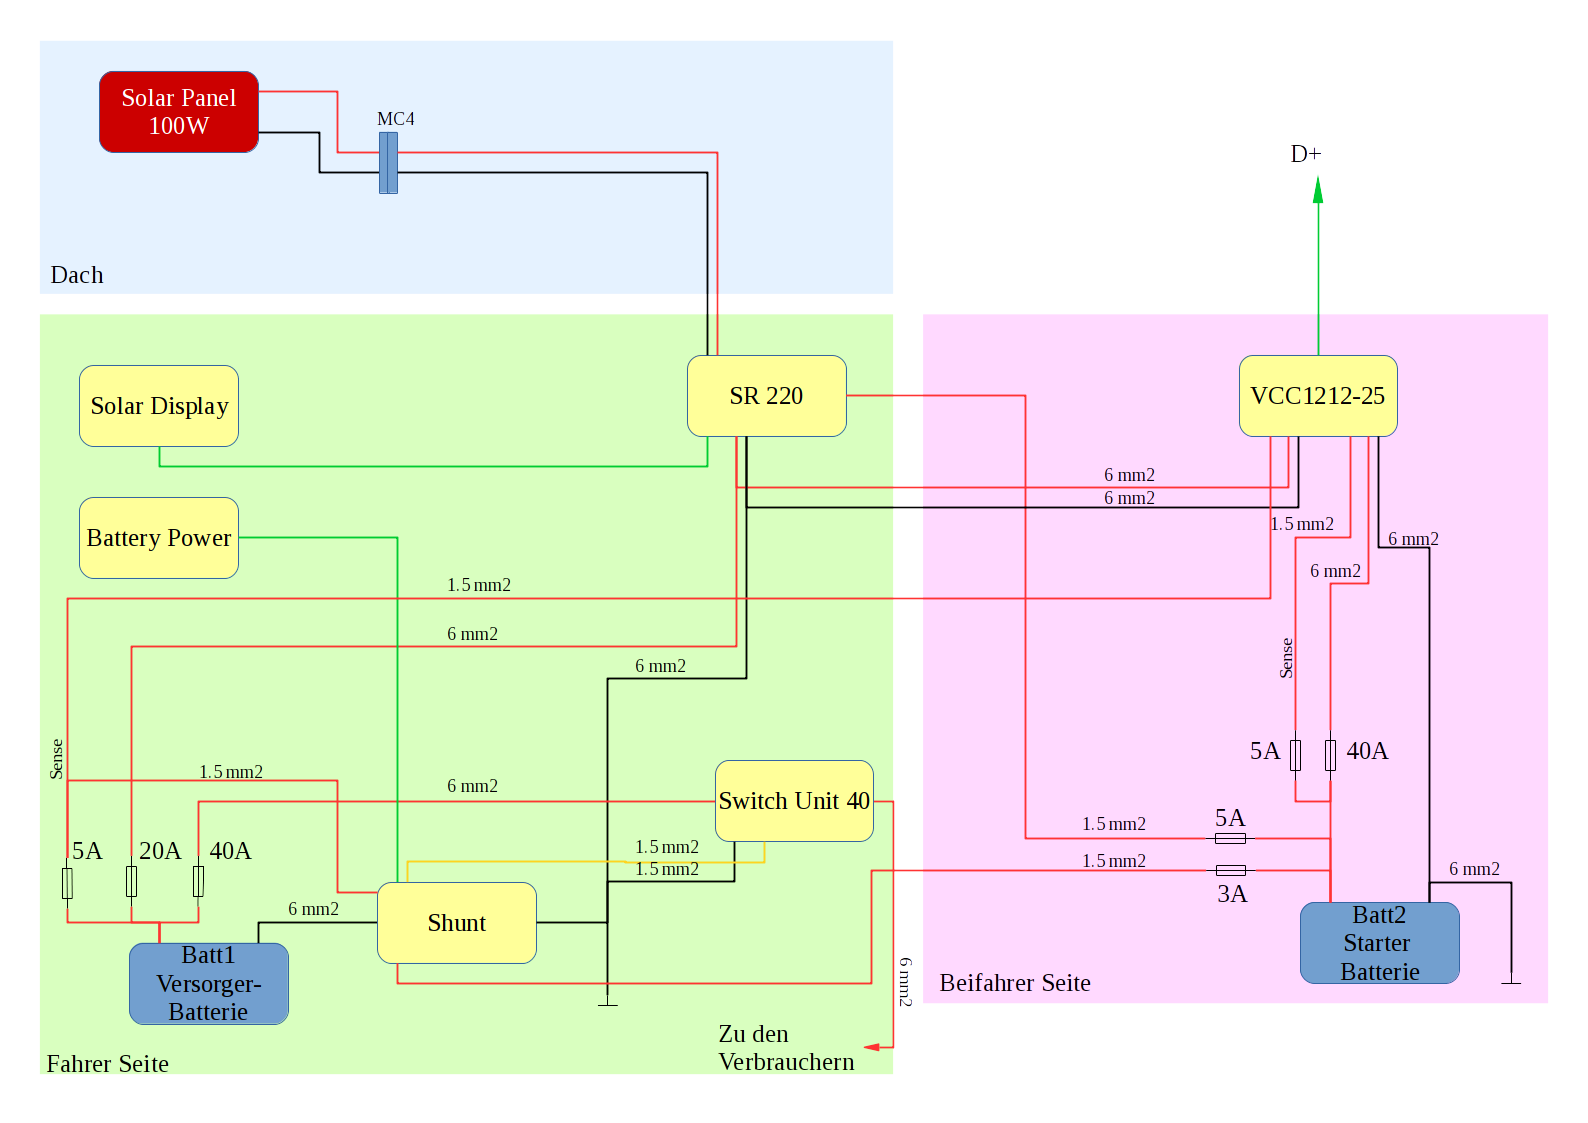
\includegraphics[scale=0.3, angle=90]{../Bilder/Anleitung/EL_System.png}
	\caption{Übersicht über das elektrische System}
	\label{Schema}
\end{figure}

\subsection{Übersicht der Bedienung}
\begin{figure}[H]
	\centering
    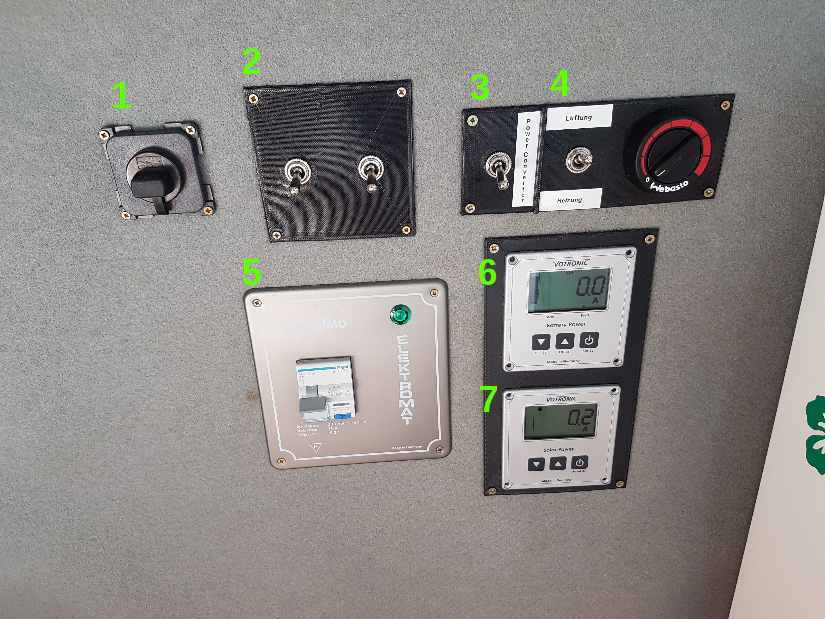
\includegraphics[width=0.8\textwidth]{../Bilder/Anleitung/Bedienung.png}
	\caption{Elektrisches Bedienpanel in der linken Seitenwand}
    \label{Bedienpanel}
\end{figure}

In der linken Seitenwand befindet sich die Bedienung der Batterieversorgung, Solaranlage, Heizung sowie die Sicherung für den 230V Anschluss.
Beschreibung der Elemente:

\begin{enumerate}
    \item USB Anschluss
    \item Lichtschalter (linker Schalter ohne Funktion)
    \item Ein-/ Auschalter für den Inverter
    \item Panel für die Standheizung
    \item Sicherung inklusive FI für den 230V Anschluss
    \item Display für die Batteriesteuerung
    \item Display für die Solarsteuerung
\end{enumerate}

\subsection{Elektronik unter dem Fahrersitz}
\begin{figure}[H]
	\centering
    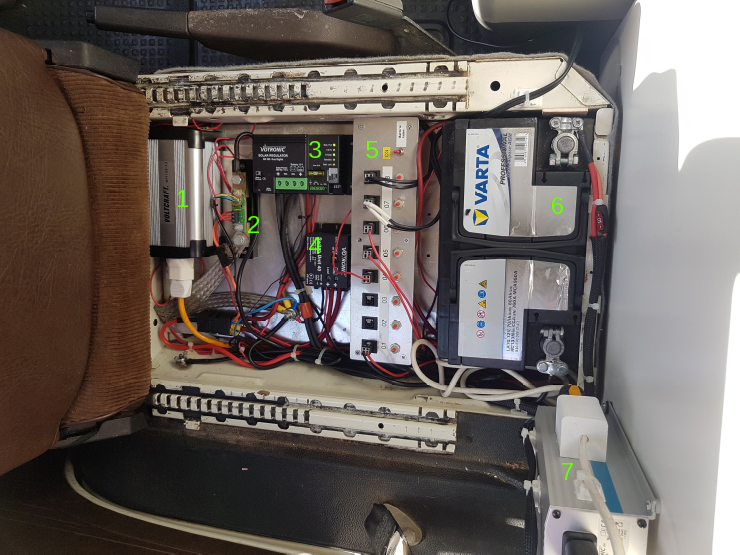
\includegraphics[width=0.8\textwidth]{../Bilder/Anleitung/Elektronik_Sitz.png}
	\caption{Elektronik unter dem Fahrersitz}
    \label{Fahrersitz}
\end{figure}

\begin{enumerate}
    \item Inverter
    \item Shunt Widerstand für die Strommessung
    \item Solarregler
    \item Switch Unit
    \item Sicherungs Panel
    \item Verbraucherbatterie
    \item 230V Batterieladegerät
\end{enumerate}

\newpage
\subsection{Solaranlage}

\subsubsection{Komponenten}
Das Solarsystem besteht aus folgenden Komponenten:

\begin{itemize}
     \item Solarpanel auf dem Dach
     \item Solarregler MPP 165 Duo Digital unter dem Fahrersitz
     \item Solardisplay in der linken Seitenwand
\end{itemize} 

(Siehe Abbildung \ref{Schema} auf Seite \pageref{Schema} für eine Gesamtübersicht)

\subsubsection{Solarpanel Wattstunde FLEX}
Auf dem Dach befindet sich ein flexibles Solarpanel, welches direkt auf das Busdach geklebt wurde

\subsubsection{Solarregler MPP 165 Duo Digital}
Unter dem Fahrersitz befindet sich ein Solarregler, welcher die von dem Solarpanel aufgefangene Energie für die Batterien aufbereitet.
Dank MPP-Funktion (Maximum Power Point) wird sichergestellt, dass eine maximale Leistungsausbeute zustanden kommt.

\subsubsection{Solardisplay in der linken Seitenwand}
Dient zur Information.
Keine Einstellungsmöglichkeiten zur Steuerung der Anlage vorhanden

\subsubsection{Bedienung und Beschreibung}
Ein 100 Watt Solarpanel auf dem Dach des Busses sorgt für die Energieversorgung falls sonst keine Energiequelle vorhanden ist. 
Für die Steuerung des Systems ist ein kleines Display (Nummer 7 in der Abbildung \ref{Bedienpanel} auf der Seite \pageref{Bedienpanel}) in der linken Seitenwand verbaut.
Es dient hauptsächlich zur Anzeige des Status der Anlage.
Das System schaltet sich automatisch ab und an, je nach dem Stand der Energiegewinnung
Falls die Batterien voll geladen sind, kann der Solarregler keine zusätzliche Energie der Batterie zufügen.
Dann kann auch bei schönstem Wetter die Stromproduktion gegen Null gehen.
Ist somit also kein Fehler der Anlage.
Das zweite Display zeigt den Ladezustand der Batterie an und kann somit zur Prüfung dienen.
Die Solaranlanlage versorgt in erster Linie die Verbraucherbatterie.
Zusätzlich wird die Starterbatterie mit bis zu 2A für die Ladungserhaltung mit geladen.
Das Solarmodul muss nicht gesteuert werden.
Das Display dient nur zu Information und wird folgendermassen bedient:

\begin{figure}[H]
	\centering
  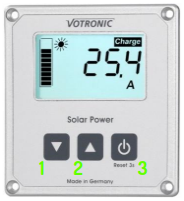
\includegraphics[width=0.5\textwidth]{../Bilder/Anleitung/Solarcomputer.png}
	\caption{Solarpanel}
    \label{Solarpanel}
\end{figure}

\begin{enumerate}
    \item Taste 1: Weiterschalten der Anzeige, Beleuchtung Einstellen (3 s)
    \item Taste 2: Zurückschalten der Anzeige, Beleuchtung Einstellen (3 s)
    \item Taste 3: Ein-/Ausschalten der Anzeige, Reset (3 s)
\end{enumerate}

Sobald oben rechts im Display das \glqq Charge\grqq{} Symbol angezeigt wird, fliesst Strom von der Solaranlage an die Batterien

\newpage
\subsection{Batterie Management}
\subsubsection{Komponenten}
\begin{itemize}
     \item Verbraucherbatterie
     \item Starterbatterie
     \item Shunt Widerstand
     \item Switch Unit 40
     \item Battery Power Display
\end{itemize} 

(Siehe Abbildung \ref{Schema} auf Seite \pageref{Schema} für eine Gesamtübersicht)

\subsubsection{Verbraucherbatterie}
Die Verbraucherbatterie versorgt alle elektrischen Verbraucher welche nicht für das Fahren des Busses gebraucht werden.
Es handelt sich dabei um eine 12V Gel Batterie, welche für die Entnahme von kleinen Strömen geeignet ist.
Die Kapazität der Batterie beträgt 70Ah.
In Verbindung mit den verschiedenen Ladeoptionen kann so die Grundversorgung sehr gut gewährleistet werden.
Es gibt drei verschiedene Arten die Batterie zu laden:

\begin{enumerate}
\item Die Solaranlage 
\item Das Batterieladegerät (230V)
\item Das Batterie zu Batterieladegerät
\end{enumerate}

Dieser Aufbau ermöglicht eine kontinuierliche Stromversorgung.
Während dem Fahren wird die Batterie über das Batterie zu Batterieladegerät geladen, auf dem Campinplatz wird mittels 230V die Batterie geladen und sobald die Sonne scheint, lädt das Solarpanel mit maximum 70 W die Batterie. 
Es sollte also immer genügend Strom vorhanden sein.

\subsubsection{Starterbatterie}
Die Starterbatterie dient in erster Linie zum Starten des Busses.
Zusätzlich werden darüber die elektrischen Verbraucher des Busses mit Energie versorgt (Licht, normale Innenraumbeleuchtung, Lüftung und Scheibenwischer).

\subsubsection{Shunt Widerstand}
Um die verbleibende Kapazität der Batterie zu errechnen ist es notwendig die entnommene Energiemenge zu kennen.
Das wird über einen Shunt Widerstand gemacht.
Diese Strommessung misst alle ein- und ausgehenden Ströme der Verbraucherbatterie.
Zusätzlich wird die Spannung der beiden Batterien gemessen. 

\subsubsection{Switch Unit 40}
Die Switch Unit dient zu Trennung der Verbaucher von der Verbraucherbatterie.
Dadurch kann die Verbraucherbatterie vor Beschädigung geschützt werden.
Die Steuerung dieses Relais geschieht über das Battery Power Display.

\subsubsection{Battery Power Display}
Alle Informationen der Batterien werden hier angezeigt. Das Panel ist in der linken Seitenwand eingebaut. (Siehe Nr. 6 auf der  Abbildung \ref{Bedienpanel})

\subsubsection{Bedienung und Beschreibung}
Das Batterie Management System dient zum Steuern, Schutz und zur Überwachung der Batterie.
Bei langer Standzeit, werden über das Display die Verbraucher von der Batterie getrennt.
Wird also der Bus aus der Tiefgarage geholt, ist zuerst die Versorgung einzuschalten.
Der Bus lässt sich auch ohne Zuschalten der Verbraucherbatterie betreiben, jedoch funktioniert das Radio, die Kühltruhe und etliche andere elektrisch betriebene Sachen nicht.
So funktioniert das Zu- und Wegschalten der Verbraucherbatterie:

\begin{figure}[H]
	\centering
  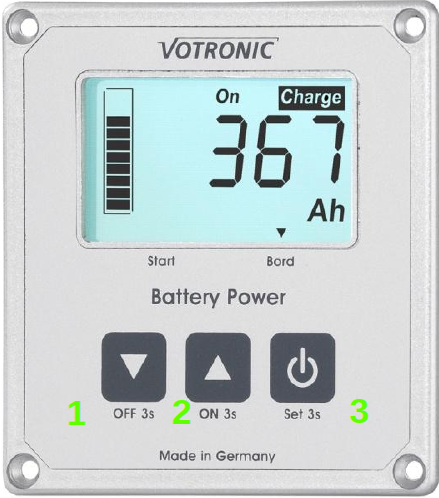
\includegraphics[width=0.5\textwidth]{../Bilder/Anleitung/Batteriecomputer.png}
	\caption{Batteriecomputer}
    \label{Batteriecomputer}
\end{figure}


\begin{itemize}
    \item Einschalten: drei Sekunden auf Taste 2 drücken
    \item Ausschalten: drei Sekunden auf Taste 1 drücken
    \item Mittels kurzem Druck auf die Taste 1 oder 2 kann durch die verschiedenen Anzeigen geschaltet werden:
    \begin{itemize}
        \item Spannung der Verbraucherbatterie
        \item Spannung der Starterbatterie
        \item Strom der Verbraucherbatterie
        \item Restlaufzeitanzeige
        \item Kapazitätsanzeige in Ah
        \item Kapazitätsanzeige in \%
    \end{itemize}
\end{itemize}

Wird eine bestimmte Reskapazität unterschritten, werden die Verbraucher von der Batterie getrennt um die Batterie zu schützen.
\subsubsection{Manueller Override}
Es gibt die Möglichkeit, das Relais manuell, ohne Display zu schalten. Nur notwendig falls das Display nicht funktioniert.

\begin{figure}[H]
	\centering
  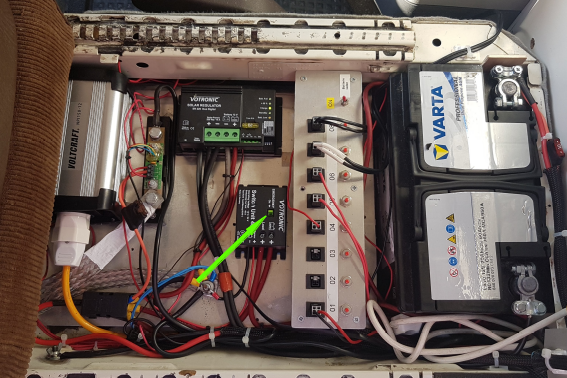
\includegraphics[width=0.8\textwidth]{../Bilder/Anleitung/Emergency.png}
	\caption{Position des manuellen Override}
    \label{Manueller Override}
\end{figure}

\subsection{Batterie zu Batterie Ladegerät}
Ein  Batterie zu Batterieladegerät befindet sich unter dem Beifahrersitz.
Dieses lädt die Verbraucherbatterie sobald der Motor läuft.
Gesteuert wird das Ladegerät über das Buseigene D+ Signal.
Das System steuert sich selbst, es ist keine Interaktion notwendig.
Ob dieses Ladegerät funktioniert, kann auf dem Battery Power Display abgelesen werden. 

\subsection{230V zu Batterie}
Das Ladegerät befindet sich am Küchenmöbel hinter dem Fahrersitz (Siehe Abbildung \ref{Fahrersitz} auf Seite \pageref{Fahrersitz})
So bald 230V über die neben dem Nummernschild angebrachten Stecker anliegen, werden beide Batterien über ein 230V zu 12V Ladegerät geladen.
Die Starterbatterie wird dabei wie bei der Ladung über das Solardach nur mit max 2A geladen.
Die Verbraucherbatterie wird mit bis zu 10A geladen.
Auch bei diesem System ist keine Aktion von Seiten Benutzer nötig. 
Der aktuelle Ladestatus kann auf dem Battery Power Display abgelesen werden.


\subsection{230V Steckdose und Anschluss im Innenraum}
Neben dem hinteren Nummernschild befindet sich unter einer Schutzkappe eine CEE Steckdose.

\begin{figure}[H]
	\centering
  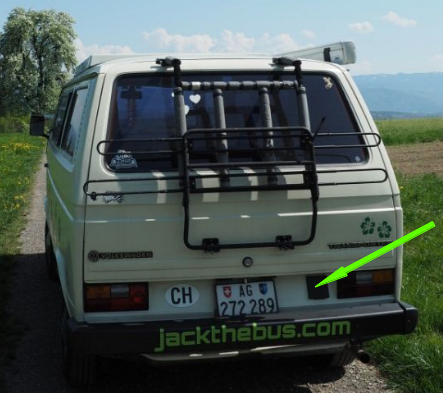
\includegraphics[width=0.6\textwidth]{../Bilder/Anleitung/Steckdose.png}
	\caption{Position der CEE Steckdose}
    \label{Steckdose}
\end{figure}

Ein Kabel (beidseitig mit CEE Stecker / Buchse) befindet sich unter der Sitzbank.
Zusätzlich ist da ein kurzes Übergangsstück mit einem (Schweizer) Typ 13 Stecker zu finden.
Falls das Kabel nicht reichen sollte, ist unter der Sitzbank noch eine kleine Kabelrolle verstaut.
Sobald Spannung am Anschluss anliegt, leuchtet im Bus die kleine grüne Kontrollleuchte neben dem FI/FL Schalter (Siehe 5 in Abbildung \ref{Bedienpanel} auf der Seite \pageref{Bedienpanel})
In diesem Stadium werden die Batterien bereits über das Ladegerät geladen.
Wird nun der FI/FL Schalter eingeschaltet (Hebelchen nach oben) ist auf der weissen 3-fach 230V Steckdose im Innenraum Strom. 
Dieser Anschluss kann gleich wie zu Hause verwendet werden.
In einem Fehlerfall würde der Stromkreis durch den FI/LS getrennt.
Um das Kabel nach Gebrauch wieder aus der CEE Steckdose zu entfernen, muss die \textbf{Verriegelung} zuerst gelöst werden (Siehe Abbildung \ref{CEE})

\begin{figure}[H]
	\centering
  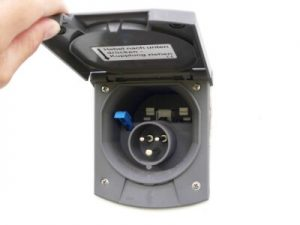
\includegraphics[width=0.6\textwidth]{../Bilder/Anleitung/CEE.jpg}
  \caption{Links oben ist die Verriegelung (blau) zu sehen}
    \label{CEE}
\end{figure}

\subsection{Inverter}
Der Inverter dient dazu den Gleichstrom der Batterie in eine Wechselstrom ähnliche Form zu bringen.
Das ermöglicht es, auch 230V Geräte im Bus zu verwenden, wenn kein Anschluss vom Campingplatz verfügbar ist.
Der verbaute Inverter liefert eine maximale Leistung von 100W.
Dies reicht für Ladegeräte oder andere kleine Verbraucher.
Haarföhn, Heizungen oder Kaffeemaschinen lassen sich jedoch nicht daran betreiben.
In der linken Seitenwand befindet sich eine einzelne schwarze Steckdose.
Nur diese wird über den Inverter versorgt.
Um den Inverter Einzuschalten, muss der Schalter für den Inverter nach oben gedrückt werden (Siehe 3 in Abbildung \ref{Bedienpanel} auf der Seite \pageref{Bedienpanel})
Es gibt Geräte welche nicht mit dem Konverter kompatibel sind. 
Der Inverter erzeugt nur ein sinusähnliches Signal welches nicht alle Verbraucher akzeptieren.
Ist dies der Fall, gibt es nur die Lösung welche im vorherigen Kapitel beschrieben worden ist.

\subsection{USB Anschluss}
Neben den Lichtaschaltern  (Siehe 1 in Abbildung \ref{Bedienpanel} auf der Seite \pageref{Bedienpanel}) befindet sich ein USB Anschluss, welcher von der Versorgerbatterie gespeist wird.
Über diesen Anschluss ist es möglich Geräte zu Laden/Betreiben. Der Ladestrom beschränkt sich auf (TBD)

\subsection{12V Anschlüsse}
Neben dem Schrank auf der Fahrerseite befinden sich knapp über dem Boden 3 12V Anschlüsse.
Wie der USB Anschluss werden diese von der Verbraucherbattere gespeist und sind somit zu Verfügung, sobald der Hauptschalter eingeschaltet wird. 
Darin können die bekannten Autoladegeräte eingesteckt werden.
Vorsichtig sollte man dann jeodch mit den Tür des Schrankes umgehen, da sonst die Stecker beschädigt werden können.

\subsection{Licht}
Alle Lichter welche sich nicht im "Fahrerhaus" befinden, werden durch die Versorgerbatterie versorgt.
Die Lampen über der Fahrer-und Beifahrertüre werden jedoch von der Starterbatterie versorgt und sollten aus diesem Grund nicht für die längerfristige Beleuchtung eingesetzt werden.
Die Beleuchtung ist im Moment Gegenstand von wilden Umbauten.
Im Moment sind diese Lampen verfügbar:
\subsubsection{Wohnraumbeleuchtung}
Über dem Ausstellfenster befindet sich eine LED Lampe in zylindrischer Bauform.
Diese kann über den rechten Schalter auf dem Panel (2) Siehe Abbildung \ref{Bedienpanel} auf Seite \pageref{Bedienpanel} ein- und ausgeschaltet werden. 
Die Lampe selbst ist drehbar um das Licht eher indirekt oder direkt im Wohnraum zu verteilen.

\subsubsection{Leselampen}
Der Bus wurde so designet, dass der Kopf beim Schlafen Richtung Heck ausgerichtet ist.
Auf beiden Seiten der Heckklappe befinden sich Leselampen, welche frei in der Ausrichtung angepasst werden können.
Der Schalter für diese Lampen ist auf dem jeweiligen Sockel der Lampe selbst angebracht.
\subsection{Sicherungen}
Inhalt
\subsection{Ersatzsicherungen}
Inhalt
\section{Elektroheizung}
Im Winter oder in der Übergangszeit, kann es schnell relativ kühl im Bus werden. 
Die eingebaute Standheizung hilft diese unangenehme Situation zu korrigieren. 
Jedoch ist der Einsatz dieser Heizung mit Emissionen (Lärm und Gestank) verbunden.
Zusätzlich wird die Batterie durch den Einsatz des Lüfters, welche für die Standheizung gebraucht wird entladen.
Wird auf einem Zeltplatz mit Stromanschluss übernachtet, besteht die Möglichkeit mittels kleiner Elektroheizung zu heizen.
Die kleine Keramikheizung befindet sich unter der Klappsitzbank und kann nachher in der weissen 230V Mehrfachsteckdose eingesteckt werden. Siehe Abbildung (TBD)
Auf keinen Fall soll versucht werden die schwarze Steckdose für den Betrieb der Elektroheizung zu verwenden.
Die Leistung des Inverters reicht bei weitem nicht für den Betrieb der Keramikheizung aus.

\section{Standheizung}
Unter dem Bus ist eine Webasto Standheizung verbaut.
Falls kein Strom zu Verfügung ist, kann trotzdem mit Hilfe von Benzin aus dem Tank des Busses und Strom aus der Versorgerbatterie Wärme generiert werden.
Der limitierende Faktor bei der Heizung ist viel weniger der Verbrauch von Benzin denn der Verbrauch von Strom aus der Batterie.

\subsection{Heizen}
Inhalt
\subsection{Lüften}
Inhalt
\subsection{Fehlercodes}
Inhalt.
\subsection{Reset}
Inhalt
\section{Kühltruhe}
Inhalt
\section{Wasser}
Inhalt
\subsection{Wasserpumpe}
Inhalt
\subsection{Abwasser}
Inhalt
\subsection{Frischwasser Kanister}
Inhalt
\section{Kochen}
Inhalt
\subsection{Küchenutensilien}
Inhalt
\section{Radio}
Inhalt
\subsection{Mit eingeschalteter Zündung}
Inhalt
\subsection{Betrieb ohne Zündung}
Inhalt
\section{Pneu Wechsel}
Das Ersatzrad des VW Buses befindet sich unter dem Fahrer und Beifahrer unter dem Bus. 
Das Rad ist von der Vorderseite her zugänglich und liegt in einer Wanne.
Um die Wanne absenken zu können um das Rad zu entnehmen, muss die Halteschraube gelöst werden und die Sicherungsklinke nach vorne gezogen werden. 
Die Halteschraube kann mit dem Radschlüssel gelöst werden, dieser befindet sich zusammen mit dem Wagenheber unter der Sitzbank. (Siehe TBD)
Jetzt ist der Moment gekommen, um zu überpüfen, ob das Rad noch Luft hat.

\subsection{Anzugsmomente}
Die Radschrauben und Muttern werden mit einem Anzugsmoment von \textbf{180 Newtonmeter} angezogen.
\subsection{Luftdruck}
Inhalt
\section{Tanken}
Inhalt
\section{Aufstelldach}
Inhalt
\section{Klappsitzbank}
Inhalt
\section{Klapptisch}
Inhalt
\section{Markise}
Inhalt

\section{Paulchen}
Paulchen ist der offizielle Name des Heckfahradträgers für den VW Bus.
Die Version welche an Jack montiert ist bietet Platz für zwei Fahrräder.
Sind keine Fahrräder zu transportieren wird der Träger hochgeklappt und mit einem alten rostigen Band gegen herunterfallen gesichert.
Nach dem entfernen des Bandes kann der untere Teil 90° nach unten geklappt werden.
Diese stellen die beiden Schienen zu Verfügung welche die Fahrräder positioniert.
Diese Schienen sind mittels Werkzeug in der Länge verstellbar.

\section{Ersatzteile}
Inhalt

\section{Werkzeug}

\begin{figure}[H]
	\centering
    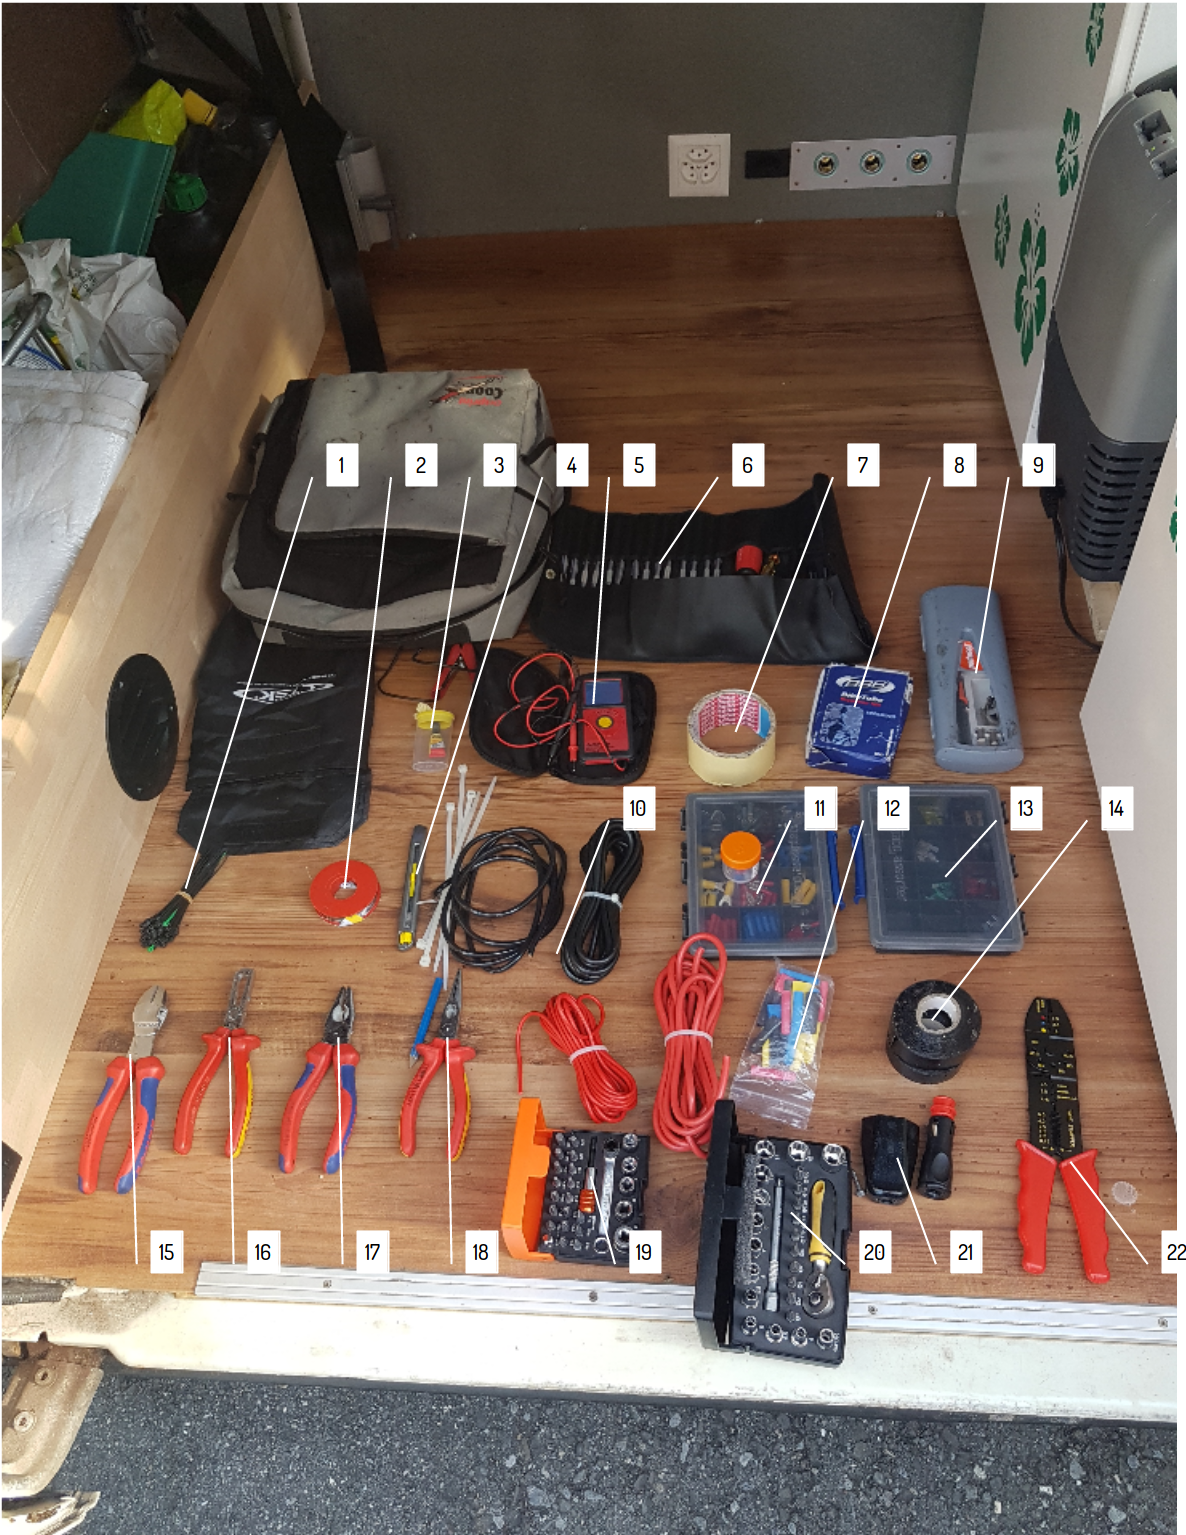
\includegraphics[width=0.95\textwidth]{../Bilder/Anleitung/Equipment_Bordwerkzeug.png}
	\caption{Bordwerkzeug}
    \label{Werkzeug}
\end{figure}

Legende zu Bild \ref{Werkzeug} auf Seite \pageref{Werkzeug}
\begin{enumerate}
    \item Kabelbinder
    \item Lötzinn
    \item Sekundenkleber
    \item Japanmesser
    \item Pocket Multimeter
    \item PB Rolltasche Schraubendreher
    \item Doppelseitiges Klebeband
    \item Ersatz Fahrradschlauch
    \item Gas Lötkolben (kann auch zum Schrumpfen verwendet werden)
    \item Diverse Kabel / Drähte
    \item Diverse Kabelverbinder und Kabelschuhe
    \item Schrumpfschlauch
    \item Sicherungssortiment
    \item Isolationsband
    \item Seitenschneider
    \item Abisolierrzange
    \item Kombizange
    \item Spitzzange
    \item Bit-Satz
    \item Ratschenschlüssel-Satz
    \item T13 Kupplung und 12V Anschluss
    \item Presszange
\end{enumerate}
All diese Gegenstände befinden sich in der grauen Tasche unter der Sitzbank
\newpage

\section{Fahrzeugausweis}
Inhalt
\section{Abgasuntersuchung}
Inhalt
\section{Versicherung}
Inhalt
\newpage
\section{TCS}
\subsection{Telefonnummern}
\begin{itemize}
    \item TCS Patrouille - Bei Panne oder Unfall in der Schweiz \\ \textbf{0800 140 140}
     \item Kundendienst 
\begin{itemize}
    \item Mo-Fr 7:30-19:00 Sa 8:00-18:00 \\ \textbf{0844 888 111}
    \item Aus dem Ausland: \\ \textbf{+41 58 827 27 27}
\end{itemize} 
\item TCS Fahrzeug-Versicherungen Mo-Fr 8:00-18:00 \\ \textbf{0800 801 000}
\item\ Einsatzzentrale ETI - Dringende Assistance-Anfragen im Ausland \\ \textbf{+41 58 827 22 20}
\item\ Adresse des Hauptsitzes \\
Touring Club Schweiz \\
Chemin de Blandonnet 4 \\
1214 Vernier \\
\textbf{0844 888 111}
\end{itemize} 

\subsection{ETI Schutzbrief}
\newpage
\section{Abläufe}
\subsection{Vor der Reise}
\subsection{Reisen}
\subsection{Aufstellen}
\subsection{Aufräumen}
\subsection{Zurückstellen}
\newpage
\section{Bekannte Mängel}
Das Alter dieses Fahrzeugs sollte nie vergessen werden. Sehr robust gebaut, ein Motor der um einiges mehr in der Lage zu leisten machen teilweise vergessen wie alt so ein Fahrzeug ist.
Das rostfreudige Material, Elektronik welche noch in den Kinderschuhen steckte und jahrelanger Schufterei tauschend mit langer Standzeit machen dem Bus das Leben schwer. 
Darum sind einige Dinge nicht mehr ganz so wie man sich das wünschen würde.
Doch genau dieser Umstand macht den VW Bus einzigartig und trägt zu seinem Mythos bei oder wie der Typ aus dem Bus Movie zu sagen pflegt:\\ \textbf{"... many human qualities, which include failures"}

\subsection{Konstantfahrruckeln}
Nervend aber ungefährlich.
Vor allem nach langen Autobahn Etappen kann es vorkommen, dass der Bus bei niedriger Drehzahl und langsamer Fahrt sich anfängt aufzuschaukeln.
Ein Gasstoss oder fahren in einem kleineren Gang helfen dagegen. Musik um im Takt mit zu wippen hilft, bei dem Geruckel nicht allzu blöd auszusehen.

\subsection{Wassereintritt in Fahrerraum}
Ein Problem welches vermeintlich schon gelöst worden ist. Je nach Lage des Busses kann es vorkommen, dass Wasser in den Fahrerraum eintritt und sich auf der Gummimatte sammelt. 
Unangenehm wenn sich da die Tasche mit der frischen Wäsche befindet. 
Eigentlich sollte das Problem behoben worden sein. 
Der Spengler hat die Scheibe mit einem frischen Gummi versehen und vorhandene Rostlöcher gestopft.
Meistens dicht.

\subsection{Auslaufen von Treibstoff beim Volltanken}
Inhalt

\subsection{Passgenauigkeit der Schlüssel}
Inhalt
\newpage
\section{Packliste}
\subsection{Allgemein}
\begin{center}
\begin{tabular}{|p{5cm}|p{5cm}|}\hline
Fotoapparat & Ladegerät Fotoapparat \\ \hline
MP3 Player & Ladegeräte Allgemein \\ \hline
Dokumente (Ausweis, Pass) & Anti Brumm \\ \hline
Linsen (Dose und Flüssigkeit) & Schlafsack \\ \hline
Kissen & Decken \\ \hline
Kleider & Schnur \\ \hline
Regenjacke & Kerzen \\ \hline
Feuerzeug & Klämmerli \\ \hline
Nastuch & Feuchttücher \\ \hline
Sackmesser & Taschenlampe \\ \hline
Stirnlampe & Reiseführer \\ \hline
Buch & Schreibzeug \\ \hline
Feldstecher & Kreditkarte \\ \hline
Krankenkasse Karte & Medikamente \\ \hline
Rucksack & Hip Bag \\ \hline
\end{tabular}
\end{center}
\newpage
 
\subsection{Küche}
\begin{center}
\begin{tabular}{|p{5cm}|p{5cm}|}\hline
Gewürze & Grill \\ \hline
Besteck & Wasserflasche \\ \hline
Gas & Grillzange  \\ \hline
Abtrocknungstuch & Abwaschmittel \\ \hline
Schokoladenpulver & Löffeli \\ \hline
Kafferahm & Schöpfkelle \\ \hline
Sieb & Tupperware \\ \hline
Abfallsäcke & kleine Plastiksäcke \\ \hline
Campinglaterne & Raco Boxen (Abwasch und Altglas) \\ \hline
Abwaschbürste & Schwamm \\ \hline
Haushaltspapier & WC Papier \\ \hline
\end{tabular}
\end{center}
\newpage

\subsection{Sommer}
\begin{center}
\begin{tabular}{|p{5cm}|p{5cm}|}\hline
Badesachen & Badetuch \\ \hline
Speedmington & Hut \\ \hline
Sonnencreme & Sonnenbrille \\ \hline
Turnschuhe & Picknickdecke \\ \hline
Stühle & Tisch \\ \hline
Sonnenschirm & Flipflop \\ \hline
\end{tabular}
\end{center}
\newpage

\subsection{Velo}
\begin{center}
\begin{tabular}{|p{5cm}|p{5cm}|}\hline
Velo Flickzeug & Velo - Bekleidung \\ \hline
Velo Schuhe & Riemen für die Befestigung der Fahrräder \\ \hline
Schloss & Pumpe \\ \hline
Navi für Velo & Bidon oder Camelback \\ \hline
Licht für den Abend & \\ \hline
\end{tabular}
\end{center}
\newpage

\subsection{Bus}
\begin{center}
\begin{tabular}{|p{5cm}|p{5cm}|}\hline
Paulchen montieren (falls nötig) & Leuchtschild für Paulchen \\ \hline
Wasserstand kontrollieren & Luftdruck kontrollieren \\ \hline
Öl Menge kontrollieren & Scheibenwaschwasserstand prüfen \\ \hline
Tanken & Reserve-Benzinkanister (je nach Land) \\ \hline
Kabelrolle und verschiedene Übergangsstecker & Zweite Kabelrolle (optional) \\ \hline
Warndreieck & Autoapotheke \\ \hline
Leuchtwesten & Ersatzrad (gepumpt!!) \\ \hline
Schlauchschellen und Kabelbinder & Klebeband \\ \hline
Eurostecker (Strom) & Werkzeug \\ \hline
Stirnlampe & Rätschensatz \\ \hline
PB Schraubenziehersatz & Lötkolben \\ \hline
Draht & Voltmeter (Batterien überprüfen) \\ \hline
\end{tabular}
\end{center}




